\chapter{飛行試験}

\section{実験の目的}
ストロー投射実験の目的はストロー単体と翼を付けた状態の飛行距離の変化を見るため行った.ストロー落下実験の目的はストローの抵抗を調べるため行った.飛行試験の実験目的は重心位置と空力中心の位置を変更した場合,飛行性能にどのような違いが発生するか調べるために

\section{実験の方法}
ストロー投射実験の実験方法はまず広い場所へ行きストローを投げる.投げた所から落ちた所までの距離を100回測り得られたデータをヒストグラムにまとめる.ストロー落下実験の実験方法は1500mmの高さからストローを落とし落下時間を計測する.この実験はストローを縦にした場合とストローを横にした場合それぞれ100回ずつ測定し得られたデータをヒストグラムにまとめる.飛行試験の実験方法はまず重心位置を変更するために先端に重量が違う重りを入れる事で重心位置を変更している.その後重心位置が重心位置より前の場合,重心位置が空力中心より後の場合,空力中心と重心位置が同じ場合の3種類の方法を試した.それぞれの方法で零戦とヘルキャットの飛行試験を100回行い得られたデータをヒストグラムにまとめる.

\section{実験結果}

\subsection{ストロー投射実験}
ストロー投下実験の結果,最大飛距離6920mm,最小飛距離2780mm,平均飛距離4150mmという結果になった.
下記にストロー投射実験から得た数値をもとに作成したヒストグラムを図(図\ref{fig:fly})に示す.

\begin{figure}[htbp]
  \begin{center}
    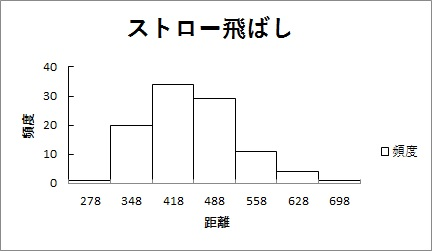
\includegraphics[width=90mm]{fly.JPG}
    \end{center}
  \caption{ストロー投射実験}
 \label{fig:fly}
\end{figure}

\subsection{ストロー落下実験横}
ストロー落下実験横の結果,最長時間0.89s,最短時間0.60s,平均時間0.75sという結果になった.
下記にストロー落下実験横から得た数値をもとに作成したヒストグラムを図(図\ref{fig:wide})に示す.

\begin{figure}[htbp]
  \begin{center}
    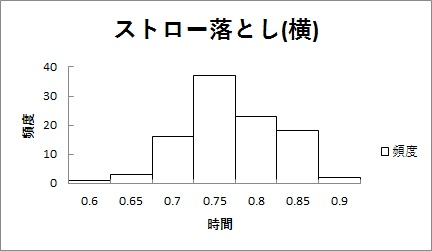
\includegraphics[width=90mm]{wide.JPG}
    \end{center}
  \caption{ストロー落下実験横}
 \label{fig:wide}
\end{figure}

\subsection{ストロー落下実験縦}
ストロー落下実験縦の結果,最長時間0.78s,最短時間0.47s,平均時間0.62sという結果になった.
下記にストロー落下実験縦から得た数値をもとに作成したヒストグラムを図(図\ref{fig:vertical})に示す.

\begin{figure}[htbp]
  \begin{center}
    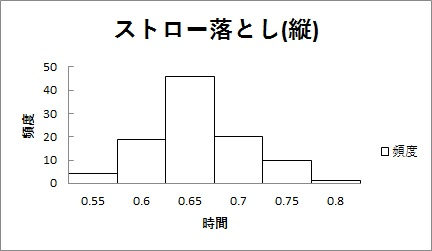
\includegraphics[width=90mm]{vertical.JPG}
    \end{center}
  \caption{ストロー落下実験縦}
 \label{fig:vertical}
\end{figure}

\subsection{重心位置が空力中心より前の場合}
\subsubsection{零戦}
重心位置が空力中心より10mm前の場合の零戦の飛行試験を行った結果,最大飛距離10060mm,最小飛距離4050mm,平均飛距離6101mmという結果になった.
下記に重心位置が空力中心より前の場合の零戦の飛行試験から得た数値をもとに作成したヒストグラムを図(図\ref{fig:zm})に示す.

\begin{figure}[htbp]
  \begin{center}
    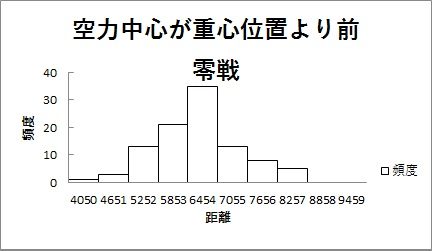
\includegraphics[width=90mm]{zm.JPG}
    \end{center}
  \caption{重心位置が空力中心より前の場合 零戦}
 \label{fig:zm}
\end{figure}

\subsubsection{ヘルキャット}
重心位置が空力中心より10mm前の場合のヘルキャットの飛行試験を行った結果,最大飛距離10040mm,最小飛距離4020mm,平均飛距離6090mmという結果になった.
下記に重心位置が空力中心より前の場合のヘルキャットの飛行試験から得た数値をもとに作成したヒストグラムを図(図\ref{fig:gm})に示す.

\begin{figure}[htbp]
  \begin{center}
    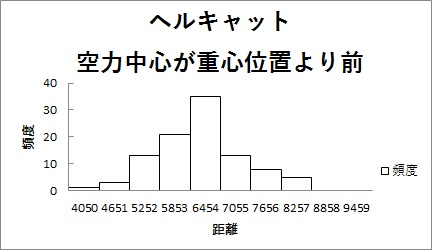
\includegraphics[width=90mm]{gm.JPG}
    \end{center}
  \caption{重心位置が空力中心より前の場合 ヘルキャット}
 \label{fig:gm}
\end{figure}

\subsection{重心位置が空力中心より後の場合}

\subsubsection{零戦}
重心位置が空力中心より7mm後の場合の零戦の飛行試験を行った結果,最大飛距離11040mm,最小飛距離4400mm,平均飛距離7250mmという結果になった.
下記に重心位置が空力中心より後の場合の零戦の飛行試験から得た数値をもとに作成したヒストグラムを図(図\ref{fig:zu})に示す.

\begin{figure}[htbp]
  \begin{center}
    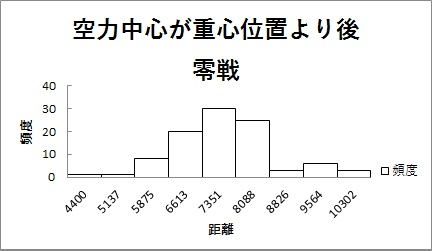
\includegraphics[width=90mm]{zu.JPG}
    \end{center}
  \caption{空力中心が重心位置より後の場合 零戦}
 \label{fig:zu}
\end{figure}

\subsubsection{ヘルキャット}
重心位置が空力中心より5mm後の場合のヘルキャットの飛行試験を行った結果,最大飛距離9510mm,最小飛距離4210mm,平均飛距離6650mmという結果になった.
下記に重心位置が空力中心より後の場合のヘルキャットの飛行試験から得た数値をもとに作成したヒストグラムを図(図\ref{fig:gu})に示す.

\begin{figure}[htbp]
  \begin{center}
    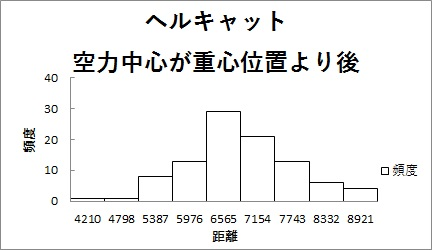
\includegraphics[width=90mm]{gu.JPG}
    \end{center}
  \caption{空力中心が重心位置より後の場合 ヘルキャット}
 \label{fig:gu}
\end{figure}

\subsection{重心位置と空力中心が同じ場合}

\subsubsection{零戦}
重心位置が重心位置が空力中心と同じ場合の零戦の飛行試験を行った結果,最大飛距離13210mm,最小飛距離4630mm,平均飛距離8100mmという結果になった.
下記に重心位置と空力中心が同じ場合の零戦の飛行試験から得た数値をもとに作成したヒストグラムを図(図\ref{fig:zo})に示す.

\begin{figure}[htbp]
  \begin{center}
    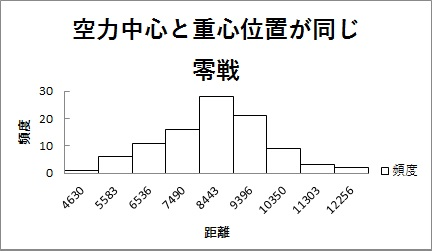
\includegraphics[width=90mm]{zo.JPG}
    \end{center}
  \caption{重心位置と空力中心が同じ場合 零戦}
 \label{fig:zo}
\end{figure}

\subsubsection{ヘルキャット}
重心位置が空力中心と同じ場合のヘルキャットの飛行試験を行った結果,最大飛距離9510mm,最小飛距離4210mm,平均飛距離6660mmという結果になった.
下記に重心位置と空力中心が同じ場合のヘルキャットの飛行試験から得た数値をもとに作成したヒストグラムを図(図\ref{fig:go})に示す.

\begin{figure}[htbp]
  \begin{center}
    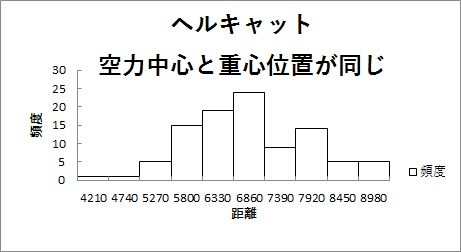
\includegraphics[width=90mm]{go.JPG}
    \end{center}
  \caption{重心位置と空力中心が同じ場合 ヘルキャット}
 \label{fig:go}
\end{figure}

\subsection{考察}
飛行試験を行った結果,ヘルキャットより零戦の方が航続距離が長いことが分かった.またストロー投射試験の平均飛距離より翼を付けた状態の機体の方が航続距離が長い.このことから翼から揚力が発生している事が分かる.
空力中心と重心位置の関係を調べた所,重心位置が空力中心より前にある場合は機体が頭上げの動作を行う,重心位置が空力中心より後にある場合は頭下げの動作を行う,重心位置と空力中心が同じ位置にある場合は頭上げ・下げの動作を行わないことが分かった.したがって重心位置と空力中心が同じ位置にある場合,理想の縦安定位置だと考える.